\PassOptionsToPackage{unicode=true}{hyperref} % options for packages loaded elsewhere
\PassOptionsToPackage{hyphens}{url}
%
\documentclass[12pt,]{report}
\usepackage{lmodern}
\usepackage{amssymb,amsmath}
\usepackage{ifxetex,ifluatex}
\usepackage{fixltx2e} % provides \textsubscript
\ifnum 0\ifxetex 1\fi\ifluatex 1\fi=0 % if pdftex
  \usepackage[T1]{fontenc}
  \usepackage[utf8]{inputenc}
  \usepackage{textcomp} % provides euro and other symbols
\else % if luatex or xelatex
  \usepackage{unicode-math}
  \defaultfontfeatures{Ligatures=TeX,Scale=MatchLowercase}
\fi
% use upquote if available, for straight quotes in verbatim environments
\IfFileExists{upquote.sty}{\usepackage{upquote}}{}
% use microtype if available
\IfFileExists{microtype.sty}{%
\usepackage[]{microtype}
\UseMicrotypeSet[protrusion]{basicmath} % disable protrusion for tt fonts
}{}
\IfFileExists{parskip.sty}{%
\usepackage{parskip}
}{% else
\setlength{\parindent}{0pt}
\setlength{\parskip}{6pt plus 2pt minus 1pt}
}
\usepackage{hyperref}
\hypersetup{
            pdftitle={Geometría analítica},
            pdfauthor={MALLQUI BAÑOS Ricardo Michel},
            pdfborder={0 0 0},
            breaklinks=true}
\urlstyle{same}  % don't use monospace font for urls
\usepackage{color}
\usepackage{fancyvrb}
\newcommand{\VerbBar}{|}
\newcommand{\VERB}{\Verb[commandchars=\\\{\}]}
\DefineVerbatimEnvironment{Highlighting}{Verbatim}{commandchars=\\\{\}}
% Add ',fontsize=\small' for more characters per line
\usepackage{framed}
\definecolor{shadecolor}{RGB}{248,248,248}
\newenvironment{Shaded}{\begin{snugshade}}{\end{snugshade}}
\newcommand{\AlertTok}[1]{\textcolor[rgb]{0.94,0.16,0.16}{#1}}
\newcommand{\AnnotationTok}[1]{\textcolor[rgb]{0.56,0.35,0.01}{\textbf{\textit{#1}}}}
\newcommand{\AttributeTok}[1]{\textcolor[rgb]{0.77,0.63,0.00}{#1}}
\newcommand{\BaseNTok}[1]{\textcolor[rgb]{0.00,0.00,0.81}{#1}}
\newcommand{\BuiltInTok}[1]{#1}
\newcommand{\CharTok}[1]{\textcolor[rgb]{0.31,0.60,0.02}{#1}}
\newcommand{\CommentTok}[1]{\textcolor[rgb]{0.56,0.35,0.01}{\textit{#1}}}
\newcommand{\CommentVarTok}[1]{\textcolor[rgb]{0.56,0.35,0.01}{\textbf{\textit{#1}}}}
\newcommand{\ConstantTok}[1]{\textcolor[rgb]{0.00,0.00,0.00}{#1}}
\newcommand{\ControlFlowTok}[1]{\textcolor[rgb]{0.13,0.29,0.53}{\textbf{#1}}}
\newcommand{\DataTypeTok}[1]{\textcolor[rgb]{0.13,0.29,0.53}{#1}}
\newcommand{\DecValTok}[1]{\textcolor[rgb]{0.00,0.00,0.81}{#1}}
\newcommand{\DocumentationTok}[1]{\textcolor[rgb]{0.56,0.35,0.01}{\textbf{\textit{#1}}}}
\newcommand{\ErrorTok}[1]{\textcolor[rgb]{0.64,0.00,0.00}{\textbf{#1}}}
\newcommand{\ExtensionTok}[1]{#1}
\newcommand{\FloatTok}[1]{\textcolor[rgb]{0.00,0.00,0.81}{#1}}
\newcommand{\FunctionTok}[1]{\textcolor[rgb]{0.00,0.00,0.00}{#1}}
\newcommand{\ImportTok}[1]{#1}
\newcommand{\InformationTok}[1]{\textcolor[rgb]{0.56,0.35,0.01}{\textbf{\textit{#1}}}}
\newcommand{\KeywordTok}[1]{\textcolor[rgb]{0.13,0.29,0.53}{\textbf{#1}}}
\newcommand{\NormalTok}[1]{#1}
\newcommand{\OperatorTok}[1]{\textcolor[rgb]{0.81,0.36,0.00}{\textbf{#1}}}
\newcommand{\OtherTok}[1]{\textcolor[rgb]{0.56,0.35,0.01}{#1}}
\newcommand{\PreprocessorTok}[1]{\textcolor[rgb]{0.56,0.35,0.01}{\textit{#1}}}
\newcommand{\RegionMarkerTok}[1]{#1}
\newcommand{\SpecialCharTok}[1]{\textcolor[rgb]{0.00,0.00,0.00}{#1}}
\newcommand{\SpecialStringTok}[1]{\textcolor[rgb]{0.31,0.60,0.02}{#1}}
\newcommand{\StringTok}[1]{\textcolor[rgb]{0.31,0.60,0.02}{#1}}
\newcommand{\VariableTok}[1]{\textcolor[rgb]{0.00,0.00,0.00}{#1}}
\newcommand{\VerbatimStringTok}[1]{\textcolor[rgb]{0.31,0.60,0.02}{#1}}
\newcommand{\WarningTok}[1]{\textcolor[rgb]{0.56,0.35,0.01}{\textbf{\textit{#1}}}}
\usepackage{longtable,booktabs}
% Fix footnotes in tables (requires footnote package)
\IfFileExists{footnote.sty}{\usepackage{footnote}\makesavenoteenv{longtable}}{}
\usepackage{graphicx,grffile}
\makeatletter
\def\maxwidth{\ifdim\Gin@nat@width>\linewidth\linewidth\else\Gin@nat@width\fi}
\def\maxheight{\ifdim\Gin@nat@height>\textheight\textheight\else\Gin@nat@height\fi}
\makeatother
% Scale images if necessary, so that they will not overflow the page
% margins by default, and it is still possible to overwrite the defaults
% using explicit options in \includegraphics[width, height, ...]{}
\setkeys{Gin}{width=\maxwidth,height=\maxheight,keepaspectratio}
\setlength{\emergencystretch}{3em}  % prevent overfull lines
\providecommand{\tightlist}{%
  \setlength{\itemsep}{0pt}\setlength{\parskip}{0pt}}
\setcounter{secnumdepth}{5}

% set default figure placement to htbp
\makeatletter
\def\fps@figure{htbp}
\makeatother

\usepackage{etoolbox}
\makeatletter
\providecommand{\subtitle}[1]{% add subtitle to \maketitle
  \apptocmd{\@title}{\par {\large #1 \par}}{}{}
}
\makeatother
\usepackage[scaled=0.92]{helvet}

\usepackage[skip=0pt]{caption}

\usepackage{sidecap}
\renewcommand{\rmdefault}{ptm}


\usepackage{amsmath}		
\usepackage[lite,subscriptcorrection,slantedGreek,nofontinfo]{mtpro2}
\usepackage{booktabs}
\usepackage{enumitem}
\usepackage[a4paper]{geometry}
\geometry{verbose,tmargin=2.5cm,bmargin=2.5cm,lmargin=3cm,rmargin=2.5cm}
\setcounter{secnumdepth}{3}
\setcounter{tocdepth}{3}
\setlength{\parindent}{2.0em}
\usepackage{color}


\usepackage{titlesec}
\newcommand{\ww}{0.015em}
\titlespacing*{\chapter}
{0pt} {5em plus \ww minus \ww} {0em plus \ww minus \ww}
\titlespacing*{\section}
{0pt} {0em plus \ww minus \ww}{0em plus \ww minus \ww}
\titlespacing*{\subsection}
{0pt} {0em plus \ww minus \ww}{0em plus \ww minus \ww}
\titlespacing*{\subsubsection}
{0pt} {0em plus \ww minus \ww}{0em plus \ww minus \ww}
\titlespacing*{\paragraph} {0pt}{1.25ex plus 1ex minus .2ex}{2em}
\titlespacing*{\subparagraph} {\parindent}{3.25ex plus 1ex minus .2ex}{1em}
\titleformat*{\section}{\normalsize\bfseries}
\titleformat*{\subsection}{\normalsize\bfseries}
\setlength{\parskip}{0.5em plus \ww minus \ww}

\titleformat{\chapter}[display]
{\normalfont\normalsize\bfseries\centering}{Capítulo \thechapter}{0.0em}{\normalsize\bfseries}
%%%%%%%%%%%%%%%%%%%%%%%%%%
\usepackage{xpatch}%space equation
\xapptocmd\normalsize{%
	\abovedisplayskip=0.5em plus \ww minus \ww
	\abovedisplayshortskip=0.5em plus \ww minus \ww
	\belowdisplayskip=0.5em plus \ww minus \ww
	\belowdisplayshortskip=0.5em plus \ww minus \ww
}{}{}
%%%%%%%%%%%%%%%%%%%%%
%\setlength\intextsep{0.5em}% plus \ww minus \ww}
\setlist{topsep=0em plus \ww minus \ww, parsep=0.5em plus \ww minus \ww, itemsep=0em} 

\setcounter{topnumber}{2}
\setcounter{bottomnumber}{2}
\setcounter{totalnumber}{4}
\renewcommand{\topfraction}{0.85}
\renewcommand{\bottomfraction}{0.85}
\renewcommand{\textfraction}{0.5}
\renewcommand{\floatpagefraction}{0.7}



\newcommand{\N}{\mathds{N}}
\newcommand{\R}{\mathds{R}}
\newcommand{\CC}{\mathds{C}}
\newcommand{\I}{\mathds{I}}
\newcommand{\f}{\mathds{f}}
\newcommand{\X}{\mathds{X}}
\newcommand{\D}{\mathds{D}}
\newcommand{\Z}{\mathds{Z}}
\newcommand{\Q}{\mathds{Q}}

\newcommand{\Ee}{\mathcal{E}}
\newcommand{\Pp}{\mathcal{P}}
\newcommand{\Ll}{\mathcal{L}}
\newcommand{\Hh}{\mathcal{H}}
\newcommand{\Cc}{\mathcal{C}}

\newcommand{\norm}[1]{\left\Vert#1\right\Vert}
\newcommand{\abs}[1]{\left\vert#1\right\vert}
\newcommand{\set}[1]{\left\{#1\right\}}
\newcommand{\seq}[1]{\left<#1\right>}
\newcommand{\co}[1]{\left[#1\right]}
\newcommand{\cc}[1]{\left(#1\right)}
% https://github.com/rstudio/rmarkdown/issues/337
\let\rmarkdownfootnote\footnote%
\def\footnote{\protect\rmarkdownfootnote}

% https://github.com/rstudio/rmarkdown/pull/252
\usepackage{titling}
\setlength{\droptitle}{-2em}

\pretitle{\vspace{\droptitle}\centering\huge}
\posttitle{\par}

\preauthor{\centering\large\emph}
\postauthor{\par}

\predate{\centering\large\emph}
\postdate{\par}
\usepackage[]{natbib}
\bibliographystyle{apalike}

\title{Geometría analítica}
\author{MALLQUI BAÑOS Ricardo Michel}
\date{2020-02-23}

\begin{document}
\maketitle

{
\setcounter{tocdepth}{1}
\tableofcontents
}
\hypertarget{algebra-vectorial}{%
\chapter{Algebra vectorial}\label{algebra-vectorial}}

\hypertarget{datos}{%
\section{Datos}\label{datos}}

Sean los datos que se prosiguen

\begin{itemize}
\tightlist
\item
  www
\item
  wwwww
\end{itemize}

\hypertarget{ff}{%
\subsection{ff}\label{ff}}

WWWW fff
WWWW wwwww

\hypertarget{ff-1}{%
\subsection{ff}\label{ff-1}}

This is a \emph{sample} book written in \textbf{Markdown}. You can use anything that Pandoc's Markdown supports, e.g., a math equation \(a^2 + b^2 = c^2_c\).

The \textbf{bookdown} package can be installed from CRAN or Github:

\begin{Shaded}
\begin{Highlighting}[]
\KeywordTok{install.packages}\NormalTok{(}\StringTok{"bookdown"}\NormalTok{)}
\CommentTok{# or the development version}
\CommentTok{# devtools::install_github("rstudio/bookdown")}
\end{Highlighting}
\end{Shaded}

Remember each Rmd file contains one and only one chapter, and a chapter is defined by the first-level heading .

To compile this example to PDF, you need XeLaTeX. You are recommended to install TinyTeX (which includes XeLaTeX): \url{https://yihui.org/tinytex/}.

\hypertarget{acciones}{%
\section{Acciones}\label{acciones}}

Sean los datos \emph{emph} \textbf{\emph{real}} \textbf{Entonces}

\hypertarget{intro}{%
\chapter{Rectas}\label{intro}}

\hypertarget{lugar-geomuxe9trico}{%
\chapter{Lugar geométrico}\label{lugar-geomuxe9trico}}

Here is a review of existing methods.

\hypertarget{circunferencia}{%
\chapter{Circunferencia}\label{circunferencia}}

Sea \(\vec{a}=(a_1,a_2)\) entonces el vector escalado es \(r\vec{a}\parallel\vec{a}\); el vector perpendicular a este es \(\vec{a}^\perp=(-a_2,a_1)\) la norma del vector \(\vec{a}\) es \(\left\|a\right\|=\sqrt{a_1^2+a_2^2}\) el vector unitario en la dirección de \(\vec{a}\) es \(\vec{\mu}=\frac{\vec{a}}{\left\|a\right\|}\) que es paralela a este. Dado dos puntos \(P_1\) y \(P_2\) estos definen un vector \(\vec{P_1P_2}=P_2-P_1\). Los vectores en dirección de los ejes positivos son \(i=(1,0)\) y \(j=(0,1)\); cualquier vector se pueden expresar en términos de estos es decir \(\vec{a}=(a_1,a_2)=a_1(1,0)+a_2(0,1)=a_1i+a_2j\). De acuerdo al ángulo de inclinación del vector se tiene la siguiente representación \(\vec{a}=\left\|\vec{a}\right\|(\cos\theta,\sin\theta)\).

Dos vectores son ortogonales (\(\vec{a}\perp\vec{b}\)) si \(\left|\vec{a}-\vec{b}\right|=\left|\vec{a}+\vec{b}\right|\) y verifican

\(\left|\vec{b}\right|^2+\left|\vec{b}\right|^2+=\left|\vec{a}+\vec{b}\right|^2\)
\(\vec{a}\vec{b}=0\)
\(\vec{a}\parallel\vec{b}^\perp\)
\(\vec{a}\) y \(\vec{b}\) son LI si y solo si \(r\vec{a}+s\vec{b}=0\) implica \(r=0\) y \(s=0\).

La proyeccion de \(\vec{a}\) sobre \(\vec{b}\) es otro vector \(\text{Proy}_{\vec{b}}\vec{a}\)

\(\vec{a}=\text{Proy}_{\vec{b}}\vec{a}+\text{Proy}_{\vec{b}^\perp}\vec{a}\) si hacemos \(\vec{a}=p\vec{b}+q\vec{b}^\perp\) entonces \(q=\frac{\vec{a}\vec{b}}{\left\|\vec{b}\right\|^2}\) y \(p=\frac{\vec{a}\vec{b}^\perp}{\left\|\vec{b}\right\|^2}\) pues \(\left\|\vec{b}\right\|=\left\|\vec{b}^\perp\right\|\) entonces \(\text{Proy}_{\vec{b}}\vec{a}=\frac{\vec{a}\vec{b}}{\left\|\vec{b}\right\|^2}\vec{b}=\frac{\vec{a}\vec{b}}{\left\|\vec{b}\right\|}\frac{\vec{b}}{\left\|\vec{b}\right\|}=\text{Cp}_{\vec{b}}\vec{a}\frac{\vec{b}}{\left\|\vec{b}\right\|}\); \(\text{Cp}_{\vec{b}}\vec{a}=\frac{\vec{a}\vec{b}}{\left\|\vec{b}\right\|}\) recibe el nombre de componente de \(\vec{a}\) en la dirección de \(\vec{b}\)

Dado \(P_0\) y un vector \(\vec{a}\) entonces la recta se define como el conjunto de puntos \(\mathcal{L}=\left\{P\in\mathbb{R}^2/P=P_0+t\vec{a};\: t\in \mathbb{R}\right\}\) que recibe el nombre de ecuación vectorial de la recta. \(P\in\mathcal{L}\iff (P-P_0)\cdot\vec{a}^\perp=0\). De la ecuación vectorial de la recta se tiene si \(P=(x.y)\); \(P_0=(x_0,y_0)\) y \(\vec{a}=(a_1,a_2)\) se tiene la ecuación paramétrica de la recta. \(x=x_0+ta_1\); \(y=y_0+ta_2\) de esto se obtiene la ecuación simétrica de la recta \[\frac{x-x_0}{a_1}=\frac{y-y_0}{a_2}.\] Sea \(\vec{n}=(a,b)=\vec{a}^\perp\) entonces se tiene que si \(P\in \mathcal{L}\) entonces \((P-P_0)\cdot \vec{n}=0\) pues son perpendicualres; entonces \(P\cdot \vec{n}=P_0\cdot \vec{n}\iff ax+by=-c\implies ax+by+c=0\) que recibe el nombre de ecuación general de la recta. Sea \(Q=(x_1,y_1)\) un punto exterior a \(\mathcal{L}\) entonces la distancia de \(Q\) a \(\mathcal{L}\) se define como

\begin{align*}d[Q;\mathcal{L}] & =\left|\text{Cp}_{\vec{n}}(Q-P_0)\right| \\
& =\left|\frac{(Q-P_0)\cdot\vec{n}}{\left|\vec{n}\right|}\right| \\
& =\left|\frac{Q\cdot\vec{n}-P_0\cdot\vec{n}}{\left|\vec{n}\right|}\right| \\
& =\frac{\left|ax_1+by_1+c\right|}{\sqrt{a^2+b^2}}
\end{align*}

Sean \(\mathcal{L}_1\) y \(\mathcal{L}_2\) dos rectas; con vectores directores \(\vec{a}=(a_1,a_2)\) y \(\vec{b}=(b_1,b_2)\) respectivamente; entonces \(\mathcal{L}_1\cap\mathcal{L}_2=(d_1,d_2)\) donde \(d_1\) y \(d_2\) satisfacen el sistema generado por las ecuaciones generales de \(\mathcal{L}_1\) y \(\mathcal{L}_2\); \(a_1x+a_1y+k_1=0\) y \(b_1x+b_1y+k_2=0\).

La pendiente de una recta se deduce de su vector director es decir si \(\vec{a}=(a_1,a_2)\) entonces \(m=\frac{a_2}{a_1}\); de esto se deduce \(\vec{a}=(a_1,a_2)=a_1(1,\frac{a_2}{a_1})=a_1(1,m)\). El angulo generado por las \(\mathcal{L}_1\) con pendiente \(m_1\) y \(\mathcal{L}_2\) con pendiente \(m_1\); está dada por \(\theta=\arctan\left(\frac{m_1-m_2}{1+m_1m_2}\right)\).

El círculo se define como el conjunto de punto \(P=(x,y)\) que satisfacen la ecuación \[\left \|P-C\right\|=r\] \(r>0\) es el radio, \(C=(h,k)\) es el centro entonces la ecuación del círculo es \[\left \|P-C\right\|=r\iff (x-h)^2+(y-k)^2=r^2.\]

La ecuación de la recta tangente en \(P_0=(x_0,y_0)\) (\(P=P_0\) en el gráfico) está dada por \[(Q-P_0)\cdot(P_0-C)=0\] donde \(Q=(x,y)\neq P\) cualquiera; entonces \[(Q-P_0)\cdot(P_0-C)=0\iff  (x-x_0,y-y_0)(x_0-h,y_0-k)=0\] lo cual es equivalente a \[(x-h)(x_0-h)+(x-k)(y_0-k)=r^2\]

\hypertarget{paruxe1bolas}{%
\chapter{Parábolas}\label{paruxe1bolas}}

Sean la recta \(\mathcal{L}\) y el punto \(F\) fijos; los puntos \(P\) que satisfacen \[d\left[P;F\right]=d\left[P;\mathcal{L}\right]=\left|p\right|\] la excentricidad es el cociente de estas dos distancias igual a \(1\).

\(\mathcal{L}\) es la recta directriz cuya ecuación es \(x'=-p\); \(F\) es el foco; \(V=(h,k)\) vértice, \(p\) parámetro de la parábola ; \(RR'\) lado recto de la parábola.

\(P=(x,y)=V+x'\vec{u}+y'\vec{u}^\perp\) \(x'=[(x,y)-V]\vec{u}\) y \(y'=[(x,y)-V]\vec{u}^\perp\)

\(\mathcal{L}=\left\{Q/Q=(V-p\vec{u})+t\vec{u}^\perp,\:t\in \mathbb{R}\right\}\); \(F=V+p\vec{u}\) luego \[d[P;\mathcal{L}]=\left|\text{Cp}_{\vec{u}}\vec{PQ}\right|=\left|(Q-P)\cdot\vec{u}\right|=\left|x'+p\right|\]

\[d[P;F]=\left|P-F\right|=\left|(x'-p)\vec{u}+y'\vec{u}^\perp\right|\] por lo tanto

\begin{align*}
d\left[P;F\right]^2=d\left[P;\mathcal{L}\right]^2
& \implies \left|(x'+p)\vec{u}+y'\vec{u}^\perp\right|^2=\left|x'+p\right|^2 \\
&\implies (x'-p)^2+y'^2=(x'+p)^2\\
&\implies y'^2=4px'
\end{align*}

De este modo \(P\in\mathcal{P}\) si \(P\) satisface la ecuacion vectorial \[P=(x,y)=V+x'\vec{u}+y'\vec{u}^\perp;\: \text{donde } y'^2=4px'; \:\left|\vec{u}\right|=1\]

Cuando el eje es paralelo al eje \(x\); \(\vec{u}=i=(1,0)\) entonces \((x,y)=V+x'\vec{u}+y'\vec{u}^\perp=(h+x',k+y')\implies x'=x-h\) y \(y'=y-k\) en \$ y'\^{}2=4px'\$ resulta \((y-k)^2=4p(x-h)\) (\(y^2=4px\) si \(V\) está en el origen); entonces \(F=V+p\vec{u}=(h+p,k)\); \(\mathcal{L}: x=h-p\). Si \(p<1\) la parábola se invierte simétricamente a la directriz.

Cuando el eje es paralelo al eje \(y\); \(\vec{u}=j=(0,1)\) entonces \((x,y)=V+x'\vec{u}+y'\vec{u}^\perp=(h-y',k+x')\implies x'=y-k\) y \(y'=h-x\) en \$ y'\^{}2=4px'\$ resulta \((x-h)^2=4p(y-k)\) (\(x^2=4py\) si \(V\) está en el origen); entonces \(F=V+p\vec{u}=(h,k+p)\); \(\mathcal{L}: x=k-p\). Si \(p<1\) la parábola se invierte simétricamente a la directriz.

La ecuación de la recta tangente a \(y^2=4px\) en el punto \(P_0=(x_0,y_0)\) está dada por \(y=\frac{2p}{y_0}(x+x_0)\) y la ecuación de la recta tangente a \((y-k)^2=4p(x-h)\) en el punto \(P_0=(x_0,y_0)\) está dada por \((y_0-k)(x_0-k)=4p\left[\left(\frac{x+x_0}{2}-h\right)\right]\) similarmente la ecuación de la recta tangente a \((x-h)^2=4p(y-k)\) en el punto \(P_0=(x_0,y_0)\) está dada por \((x_0-h)(x_0-h)=4p\left[\left(\frac{y+y_0}{2}-h\right)\right]\).

\begin{enumerate}
\def\labelenumi{\arabic{enumi}.}
\item
  Al realizarse una transformacion de coordenadas, el eje de una parabola \(\mathcal{P}\) resulta orientada segun el vector \((3,4)\). En \(x'y'\) un punto \(Q'=(20,-20)'\in\mathcal{P}\) en els sistema \(xy\) el foco de \(\mathcal{P}\) \(E=(11,5)\). Determinar en el sistema \(xy\) un punto \(R\) de la parabola \(\mathcal{P}\) tal que el trinagulo \(QVR\) sea rectangulo en \(V\) vertice de la parábola.
\item
  La circunferencia \(\mathcal{C}=(x-3)^2+(y-3)^2=25\) es tangente a una parábola \(\mathcal{P}\) en \(P_0=(x_0,y_0)\), \(y_0>7\). La recta \(\mathcal{L}:4x-3y+12=0\) es normal a \(\mathcal{P}\) y \(\mathcal{C}\) en \(P_0\) y corta al eje focal de \(\mathcal{P}\) en el punto \(R\). Si \(\left|\vec{C_0P_0}\right|=\left|\vec{P_0R}\right|\) y si la distancia \(d[P_0; \text{eje focal}]=4\), hallar la ecuación de la parábola \(\mathcal{P}\). \(C_0\) es el centro de la circunferencia y la absisa del vértice es menor que 6.
\end{enumerate}

\(P_0=C_0\pm r\vec{u}_{\mathcal{L}}\) donde \(r=5\), \(C_0=(3,8)\) y \(\vec{u}_{\mathcal{L}}=\frac{(3,4)}{5}\) es decir \(P_0=(3,8)\pm 5\frac{(3,4)}{5}\) de esto consideramos \(P_0=(x_0,y_0)=(6,12)\) por condición del problema con esto la recta tangente a \(\mathcal{C}\) y \(\mathcal{P}\) es \(\mathcal{L}_T:(x,y)(3,4)=(3,4)(6,12)\) equivalentemente \(\mathcal{L}_T:3x+4y=66\).

Ya que \(\left|\vec{C_0P_0}\right|=5=\left|\vec{P_0R}\right|\) y \(d[P_0;\text{eje focal}]=d[P_0; Q]=4\) entonces el triángulo \(P_0QR\) es un triángulo rectángulo notable, por lo tanto \(\left|\vec{QR}\right|=3\) por el Teorema de Pitágoras, además \(\vec{P_0R}=\vec{P_0Q}+\vec{QR}\) es decir si \(\vec{P_0Q}=(v_1,v_2)\) se tiene la ecuacion \((3,4)=4(v_1,v_2)\pm 3(-v_2,v_1)\) que al resolverla se tiene \(\vec{P_0R}=(v_1,v_2)=(1,0)\) o \(\vec{P_0R}=(v_1,v_2)=\left(\frac{24}{25},\frac{7}{25}\right)\) entonces \(Q=P_0+4(0,1)=(6,16)\) o \(Q=P_0+4\left(\frac{24}{25},\frac{7}{25}\right)=\left(6+\frac{96}{25},12+\frac{28}{25}\right)\) esto indica considerar \(Q=(6,16)\) pues el vertice (tiene absisa menor que 6), debe estar a la derecha de \(P_0\) pues la recta \(\mathcal{L}_T\) tiene pendiente negativa. Por lo tanto \(\mathcal{L}_T\cap \mathcal{F}:x=16=(\frac{2}{3},16)\) y por propiedad de la tangente a una parábola se tiene el vértice \(V=\left(\frac{\mathcal{L}_T\cap \mathcal{F}+Q}{2}\right)=\left(\frac{10}{3}, 16\right)\). La ecuación de la parabola en le sistema original es \((y-h)^2=4\rho(x-k)\) donde \((h,k)=\left(\frac{10}{3}, 16\right)\) y \((6,12)\in\mathcal{P}\) se tiene \((-4)^2=4\rho(8/3)\) de donde \(\rho=\frac{3}{2}\) entonces la recta directriz pasa por \(\left(\frac{10}{3}, 16\right)+\frac{3}{2}(1,0)=\left(\frac{7}{3}, 16\right)\) por tanto \(\mathcal{L}_D:x=\frac{7}{3}\) y la ecuacion de la parábola es \[(y-16)^2=4\rho\left(x-\frac{10}{3}\right)\] por ser paralela al eje \(x.\)

\begin{enumerate}
\def\labelenumi{\arabic{enumi}.}
\setcounter{enumi}{1}
\tightlist
\item
  Los puntos \(A=(60,13)\) y \(B=(-4,61)\) estan sobre una parábola \(\mathcal{P}\) además son simétricos con recpecto al eje focal. Desde un punto \(Q\) sobre el eje focal se traza un recta tangente a \(\mathcal{P}\) que pasa por \(B,\) hallar la ecuación de \(\mathcal{P}\) y las ecuaciones de las rectas tangentes trazadas desde \(Q\).
\end{enumerate}

Ya que \(A\) y \(B\) son simétricas entonces \(P_0=\frac{A+B}{2}=(28,37) \in \mathcal{L}_F\) donde \(\mathcal{L}_F\) es el eje focal paralelo al vector \(\vec{AB}^\perp=(B-A)^\perp=(-64,48)\parallel(-4,3)=\vec{v}_L\) es decir \(\vec{v}_F\) y \(P_0\) nos genera la ecuación del eje focal \(\mathcal{L}_F:4x+3y=1\). De otro lado dado el punto \(Q=(20,x)\in\mathcal{L}_F\) que al reemplazarlo en la recta del eje focal nos genera \(x=-27\) de donde \(Q=(20,-27)\) ademas el vértice de la parabola es \(V=\frac{Q+P_0}{2}=(4,5)\) por propiedad.

Con el objetivo de hallar el valor de \(\rho\) en la ecuación \(y'^2=4\rho x'\) se halla las coordenadas de \(B\) en el nuevo sistema de coordenadas centrada en \(V\) con vector director \(\vec{u}=\frac{(3,4)}{5}\), haciendo uso de la relación \[(x,y)=V+x'\vec{u}+y'\vec{u}^\perp\] se obtiene \(x'=\left[B-V\right]\vec{u}=40\) y \(y'=\left[B-V\right]\vec{u}^\perp=40\) por tanto reemplazando \(B=(-4,61)=(40,40)'\) en \(y'^2=4\rho x'\) se tiene que \(\rho=10\)

Los vectores directores de las rectas tangentes en el sistema \(x'y'\) son \((2,1)\) y \((2,-1)\) respectivamente por tanto sus ecuaciones son \(\mathcal{L}_A: 2y'=x'+40\) y \(\mathcal{L}_B=-2y'=x'+40\) estas ecuaciones en el sistema original con \(x'=\left[(x,y)-(4,5)\right]\frac{(3,4)}{5}\) y \(y'=\left[(x,y)-(4,5)\right]\frac{(-4,3)}{5}\) reemplazadas resultan \(\mathcal{L}_A:2y-11x-166=0\) y \(\mathcal{L}_B:5x-10y-170=0\)

\begin{enumerate}
\def\labelenumi{\arabic{enumi}.}
\tightlist
\item
  ww
\end{enumerate}

\hypertarget{elipse}{%
\chapter{Elipse}\label{elipse}}

Dados dos puntos distintos \(F_1\) y \(F_2\) llamados focos; la elipse \(\mathcal{E}\) es el conjunto formado por los puntos \(P\) que satisfacen la ecuacion \[\left|P-F_1\right|+\left|P-F_2\right|=2a.\]

\(C=(h,k)\) es el centro de la elipse; \(x'\) eje focal, \(V_1\) y \(V_2\) son los vértices de la elipse; \(\overline{V_1V_2}\) el eje mayor \(\overline{RR'}\) el lado recto; \(\overline{B_1B_2}\) el eje menor de longitud \(2b\). En el sistema \(x'y'\) se tiene \(B_1=(0,b)'\); \(B_2=(0,-b)'\); \(F_1=(-c,0)'\); \(F_2=(c,0)'\) y \(C=(0,0)'\).

\begin{figure}

{\centering 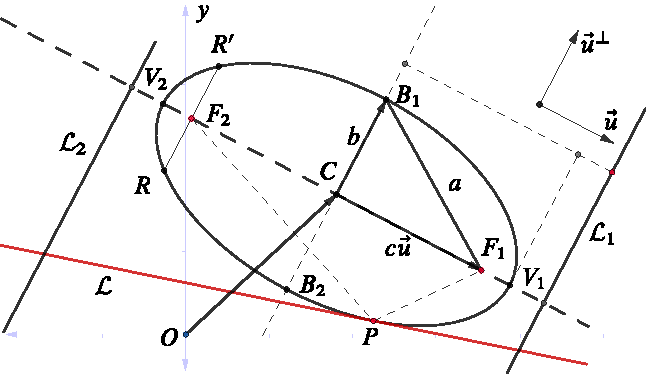
\includegraphics{elipse} 

}

\caption{Elipse vectorial}\label{fig:pressure1}
\end{figure}

La excentricidad \(e\) se define como

\[\frac{d\left[P;F_1\right]}{d\left[P;\mathcal{L}_1\right]}=e=\frac{d\left[P;F_2\right]}{d\left[P;\mathcal{L}_2\right]}\]

\(d\left[B_i;F_1\right]=d\left[B_i;F_2\right]= a\) y \(d\left[V_i;C\right]=d\left[V_i;C\right]=a\), \(i=1,2\). \(d\left[C;;\mathcal{L}_1\right]=d\left[C;\mathcal{L}_2\right]=\frac{a}{e}\) pues \(\frac{d\left[B_i;F_1\right]}{d\left[B_i;\mathcal{L}_1\right]}=e\implies \frac{a}{d\left[B;\mathcal{L}_1\right]}=e\). Sea \(c=d\left[P;F_1\right]=d\left[P;F_2\right]\implies c=ae\) pues \(\frac{d\left[P;F_1\right]}{d\left[P;\mathcal{L}_1\right]}=e\implies \frac{a-c}{\frac{a}{e}-a}=e \implies c=ae\). \(a>b\) y \(a^2=b^2+c^2\); pues \(a=d\left[B_1;F_2\right]=d\left[(0,b^2+c^2)';(c,0)'\right]^2=\sqrt{b}\); \(0<e<1\) debido a que \(0<e=\frac{a}{e}<1\) y \(a>c>0\).

\(P=(x,y)=C+x'\vec{u}+y'\vec{u}^\perp\); \(x'=[(x,y)-C]\vec{u}\); \(y'=[(x,y)-C]\vec{u}^\perp\)

\(F_1=C+c\vec{u}\) y \(F_2=C-c\vec{u}\) entonces

\begin{align*}
\left|P-F_1\right|+\left|P-F_2\right|&=\left|C+x'\vec{u}+y'\vec{u}^\perp-C+c\vec{u}\right|\\
&\quad+\left|C+x'\vec{u}+y'\vec{u}^\perp-C-c\vec{u}\right|\\
&=\sqrt{(x'+c)^2+y'^2}+\sqrt{(x'-c)^2+y'^2}=2a\end{align*}

por lo tanto resolviendo \(\sqrt{(x'+c)^2+y'^2}+\sqrt{(x'-c)^2+y'^2}=2a\) resulta \((a^2-c^2)x'^2+ay'^2=a^2(a^2-c^2)\implies b^2x'^2+a^2y'^2=a^2b^2\)

De este modo \(P\in\mathcal{E}\) si \(P\) satisface la ecuación vectorial \[P=(x,y)=V+x'\vec{u}+y'\vec{u}^\perp;\: \text{donde } \frac{x'^2}{a^2}+\frac{y'^2}{b^2}=1; \:\left|\vec{u}\right|=1\]

Cuando el eje es paralelo al eje \(x\); \(\vec{u}=i=(1,0)\) entonces \((x,y)=V+x'\vec{u}+y'\vec{u}^\perp=(h+x',k+y')\implies x'=x-h\) y \(y'=y-k\) en \(\frac{x'^2}{a^2}+\frac{y'^2}{b^2}=1\) resulta \(\frac{(y-k)^2}{a^2}+\frac{(y-k)^2}{b^2}=1\) (\(\frac{x^2}{a^2}+\frac{y^2}{b^2}=1\) si \(V\) está en el origen); entonces \(F_1=C+c\vec{u}=(h+c,k)\); \(\mathcal{L}_1: x=h+\frac{a}{e}\) y \(\mathcal{L}_2: x=h-\frac{a}{e}\).

Cuando el eje es paralelo al eje \(y\); \(\vec{u}=j=(0,1)\) entonces \((x,y)=V+x'\vec{u}+y'\vec{u}^\perp=(h-y',k+x')\implies x'=y-k\) y \(y'=h-x\) en \(\frac{x'^2}{a^2}+\frac{y'^2}{b^2}=1\) resulta \(\frac{(y-k)^2}{a^2}+\frac{(y-k)^2}{b^2}=1\) (\(\frac{x^2}{a^2}+\frac{y^2}{b^2}=1\) si \(V\) está en el origen); entonces \(F_1=C+c\vec{u}=(h+c,k)\); \(\mathcal{L}_1: x=k+\frac{a}{e}\) y \(\mathcal{L}_2: x=k-\frac{a}{e}\).

\hypertarget{hiperbola}{%
\chapter{Hiperbola}\label{hiperbola}}

Los puntos de un hipérbola verifican la siguiente ecuación

\[\left|\left|P-F_1\right|+\left|P-F_1\right|\right|=2a\]

\(C=(h,k)\) es el centro de la hipérbola; \(V_1\) y \(V_2\) son los vértices; \(F_1\) y \(F_2\) son los focos; \(\overline{V_1V_2}\) es el eje transversal; \(\overline{B_1B_2}\) es el eje conjugado; \(x'\) es el eje focal

\[d\left[C;F_1\right]=d\left[C;F_2\right]=c\]

\(F_1=(-c,0)\); \(F_1=(c,0)\) en el sistema coordenado \(x'y'\); \(\mathcal{C}\) circunferencia con centro en \(C\), radio \(c\) que pasa por los focos.

\(d\left[V_1;C\right]=d\left[V_2;C\right]=a\)

\begin{figure}

{\centering 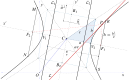
\includegraphics{hiperbola} 

}

\caption{Elipse vectorial}\label{fig:hiperbola}
\end{figure}

\[\frac{d\left[P;F_1\right]}{d\left[P;\mathcal{L}_1\right]}=e=\frac{d\left[P;F_2\right]}{d\left[P;\mathcal{L}_2\right]}\]

\(c=ae\); \(d\left[C;\mathcal{L}_1\right]=d\left[C;\mathcal{L}_2\right]=\frac{a}{e}\) y \(e>1\); en efecto \[\frac{d\left[R;F_1\right]}{d\left[R;\mathcal{L}_1\right]}=\frac{\frac{b^2}{a}}{c-d\left[C;\mathcal{L}_1\right]}=\frac{c^2-a^2}{a(c-d\left[C;\mathcal{L}_1\right])}\]

\[\frac{d\left[V_2;F_1\right]}{d\left[V_2;\mathcal{L}_1\right]}=\frac{c-a}{a-d\left[C;\mathcal{L}_2\right]}.\]

De la primera \[d\left[C;\mathcal{L}_2\right]=a-\frac{c-a}{e}\implies c-d\left[C;\mathcal{L}_2\right]=a-\frac{(c-a)(e+1)}{e}.\]

De la segunda ecuación \[c^2-a^2=ae\frac{(c-a)(e+1)}{e}\implies c+a=a(e+1)\implies c=ae\] luego \(d\left[C;\mathcal{L}_2\right]=a-\frac{(c-a)(ae+a)}{e}=\frac{a}{e}\) y el caso \(d\left[C;\mathcal{L}_1\right]\) es similar. Finalmente \(e=\frac{c}{a}>1\) pues \(0<a<c.\)

\(P=(x,y)=C+x'\vec{u}+y'\vec{u}^\perp\) \(x'=[(x,y)-C]\vec{u}\) y \(y'=[(x,y)-C]\vec{u}^\perp\)

\(F_1=C+c\vec{u}\) y \(F_2=C-c\vec{u}\) tambien \(V_1=C+a\vec{u}\) y \(V_2=C-a\vec{u}\) entonces \[\frac{d\left[P;F_1\right]}{d\left[P;\mathcal{L}_1\right]}=e\iff d\left[P;F_1\right]^2=e^2d\left[P;\mathcal{L}_1\right]^2\] haciendo uso de \(c=ae\) y \(c^2=a^2+b^2\) se tiene lo siguiente

\[(x'-c)^2+y'^2=e^2\left(x'-\left(\frac{a}{e}\right)\right)^2\]

\[(c^2-a^2) x'^2+a^2y'^2=a^2(c^2-a^2)\]

\[b^2x'^2-a^2y'^2=a^2b^2\]

De este modo \(P\in\mathcal{H}\) si \(P\) satisface la ecuación vectorial \[P=(x,y)=V+x'\vec{u}+y'\vec{u}^\perp;\: \text{donde } \frac{x'^2}{a^2}-\frac{y'^2}{b^2}=1; \:\left|\vec{u}\right|=1.\]

Cuando el eje es paralelo al eje \(x\); \(\vec{u}=i=(1,0)\) entonces \((x,y)=V+x'\vec{u}+y'\vec{u}^\perp=(h+x',k+y')\implies x'=x-h\) y \(y'=y-k\) en \(\frac{x'^2}{a^2}-\frac{y'^2}{b^2}=1\); resulta \(\frac{(y-k)^2}{a^2}-\frac{(y-k)^2}{b^2}=1\); (\(\frac{x^2}{a^2}-\frac{y^2}{b^2}=1\); si \(V\) está en el origen); entonces \(F_1=C+c\vec{u}=(h-\frac{a}{e},k)\) y \(F_2=C+c\vec{u}=(h-\frac{a}{e},k)\); \(\mathcal{L}_1: x=h-\frac{a}{e}\) y \(\mathcal{L}_2: x=h+\frac{a}{e}\) y las asíntotas de \(y'=\pm\frac{a}{b}x'\) se convierte en \((y-k)=\pm\frac{a}{b}(x-h)\).

Cuando el eje es paralelo al eje \(y\); \(\vec{u}=j=(0,1)\) entonces \((x,y)=V+x'\vec{u}+y'\vec{u}^\perp=(h-y',k+x')\implies x'=y-k\) y \(y'=h-x\) en \(\frac{x'^2}{a^2}-\frac{y'^2}{b^2}=1\); resulta \(\frac{(y-k)^2}{a^2}-\frac{(y-k)^2}{b^2}=1\); (\(\frac{x^2}{a^2}-\frac{y^2}{b^2}=1\); si \(V\) está en el origen); entonces \(F_1=C+c\vec{u}=(h+c,k)\); \(\mathcal{L}_1: x=k+\frac{a}{e}\) y \(\mathcal{L}_2: x=k-\frac{a}{e}\) y las asíntotas de \(y'=\pm\frac{b}{a}x'\) se convierte en \((y-k)=\pm\frac{b}{a}(x-h)\).

\bibliography{book.bib,packages.bib}

\end{document}
